%% This skeleton file requires IEEEtran.cls version 1.6 or later.
%%
\documentclass[conference,letterpaper]{IEEEtran}
% If the IEEEtran.cls has not been installed into the LaTeX system files,
% manually specify the path to it:
% \documentclass[conference]{../sty/IEEEtran}
\IEEEoverridecommandlockouts
\overrideIEEEmargins

% some very useful LaTeX packages include:

%\usepackage{cite}      % Written by Donald Arseneau
                        % V1.6 and later of IEEEtran pre-defines the format
                        % of the cite.sty package \cite{} output to follow
                        % that of IEEE. Loading the cite package will
                        % result in citation numbers being automatically
                        % sorted and properly "ranged". i.e.,
                        % [1], [9], [2], [7], [5], [6]
                        % (without using cite.sty)
                        % will become:
                        % [1], [2], [5]--[7], [9] (using cite.sty)
                        % cite.sty's \cite will automatically add leading
                        % space, if needed. Use cite.sty's noadjust option
                        % (cite.sty V3.8 and later) if you want to turn this
                        % off. cite.sty is already installed on most LaTeX
                        % systems. The latest version can be obtained at:
                        % http://www.ctan.org/tex-archive/macros/latex/contrib/supported/cite/

\usepackage{graphicx}  % Written by David Carlisle and Sebastian Rahtz
                        % Required if you want graphics, photos, etc.
                        % graphicx.sty is already installed on most LaTeX
                        % systems. The latest version and documentation can
                        % be obtained at:
                        % http://www.ctan.org/tex-archive/macros/latex/required/graphics/
                        % Another good source of documentation is "Using
                        % Imported Graphics in LaTeX2e" by Keith Reckdahl
                        % which can be found as esplatex.ps and epslatex.pdf
                        % at: http://www.ctan.org/tex-archive/info/

%\usepackage{amsmath}   % From the American Mathematical Society
                        % A popular package that provides many helpful commands
                        % for dealing with mathematics. Note that the AMSmath
                        % package sets \interdisplaylinepenalty to 10000 thus
                        % preventing page breaks from occurring within multiline
                        % equations. Use:
\usepackage{multirow}
%\usepackage[left=0.71in,top=0.94in,right=0.71in,bottom=1.18in]{geometry}
\setlength{\columnsep}{0.25in}
% correct bad hyphenation here
%\hyphenation{op-tical net-works semi-conduc-tor IEEEtran}


\begin{document}
% paper title
\title{\huge Preparation of Papers in Two-Column Format\\
for 2007 NECEC Proceedings}

% author names and affiliations
\author{\authorblockN{Karen Garfield and Mickey Mouse}
\authorblockA{\textit{Electrical and Computer Engineering}\\
\textit{Faculty of Engineering and Applied Science}\\
\textit{Memorial University}\\
\textit{\{kgarfield, mmouse\}@mun.ca}\\}%
\and
\authorblockN{Monkey King, Bajie Zhu, and Seng Tang}
\authorblockA{\textit{Department of Intelligent Robotics}\\
\textit{University of Huaguoshan}\\
\textit{Huaguoshan, Jileshijie Province, China}\\
\textit{monkey.king@uhuaguoshan.edu.cn}\\}}%

% make the title area
\maketitle
\begin{abstract}
These instructions give you the basic guidelines for preparing
papers for NECEC conference proceedings.
\\
\end{abstract}

% key words
\begin{keywords}
List key index terms here. No more than 5.
\end{keywords}

\section{Introduction}
% no \PARstart
Your goal is to simulate the usual appearance of papers in \textit{IEEE
conference proceedings}. For items not addressed in these
instructions, please refer to the last issue of your conference's
proceedings for reference or ask your conference Publications
Chair for instructions.

%\hfill mds
%\hfill August 13, 2002

\subsection{Preparing Your Paper}
\subsubsection{Paper Size}

Prepare your paper in full-size format on US letter size paper 
(8.5 by 11 inches).

\subsubsection{Type Sizes and Typefaces}

Follow the font type sizes specified in Table I. The font type sizes are 
given in points, same as in the MS Word font size points. Times New Roman 
is the preferred font.

\subsubsection{Paper Margins}

Paper margins on the US letter size paper are set as follows: 
top = 0.75 inches, bottom = 1 inch, side = 0.625 inches. 
Each column measures 3.5 inches wide, with a 0.25-inch gap 
between the two columns.

\subsubsection{Paper Styles}

Left- and right-justify the columns.  On the last page of your paper, 
adjust the lengths of the columns so that they are equal.  Use automatic 
hyphenation and check spelling and grammar. Use high resolution 
(300 dpi or above) figures, plots, drawings and photos for best 
printing result.

% An example of a floating table. Note that, for IEEE style tables, the
%\caption command should come BEFORE the table.Table text will default to
%\footnotesize as IEEE normally uses this smaller font for tables.
%The \label must come after \caption as always.


\begin{table}[h]
% increase table row spacing, adjust to taste
\renewcommand{\arraystretch}{1.2}
\renewcommand{\thefootnote}{\alph{footnote}}
\caption{Type Size For Papers} \label{table1}
\begin{minipage} {0.5\textwidth}
%% The array package and the MDW tools package offers better commands
%% for making tables than plain LaTeX2e's tabular which is used here.
%\bigskip
\begin{center}
\begin{tabular}{|c|p{1.25in}|p{0.98in}|p{0.45in}|}
\hline
\multirow{2}{0.1in}{\tiny{Type size (pts.)}} 
& \multicolumn{3}{|c|}{Appearance}\\
\cline{2-4}
%& \multicolumn{1}{|p{1.1in}|}{Regular}& \multicolumn{1}{|p{0.5in}|}{Bold}& \multicolumn{1}{|p{0.4in}|}{Italic}\\
& \multicolumn{1}{|c|}{Regular}& \multicolumn{1}{|c|}{Bold}& \multicolumn{1}{|c|}{Italic}\\
%&Regular & Bold & Italic\\
\hline
%\cline{2-4}
6 &  Table superscripts &  & \\
\cline{2-4}
8 &  Section titles\footnotemark\footnotetext{$^{\textmd{a}}$Uppercase}, references, tables, table names\footnotemark[1], table captions, figure captions, footnotes, text subscripts, and superscripts &  & \\
\cline{2-4}
9 &  & Abstract, Index Terms & \\
\cline{2-4}
10 &  Authors affiliations, main text, equations, first letter in section titles\footnotemark[1] &  & Subheading\\
\cline{2-4}
11 &  Authors' names &  & \\
\cline{2-4}
22 &  Paper title &  & \\
\hline
\end{tabular}
\end{center}
\end{minipage}
\end{table}

% \subsection{Preparing Your PDF Paper for IEEE Xplore\copyright}
% Detailed instructions on how to prepare PDF files of your papers for IEEE \textit{Xplore\copyright} can be found at
% \begin{center} http://www.ieee.org/pubs/confpubcenter \end{center}
% PDF job setting files for Acrobat versions 4, 5 and 6
% can be found for downloading from the
% above webpage as well. The instructions for preparing PDF
 % papers for IEEE \textit{Xplore\copyright} must be strictly followed.

\section{Helpful Hints}
% no \PARstart
\subsection{Figures and Tables}
Try to position figures and tables at the tops and bottoms of
columns and avoid placing them in the middle of columns. Large
figures and tables may span across both columns. Figure captions
should be centered below the figures; table captions should be
centered above. Avoid placing figures and tables before their
first mention in the text. Use the abbreviation "Fig. \#," even at
the beginning of a sentence.\\
\indent
Figure axis labels are often a source
of confusion. Use words rather than symbols. For example, as shown
in Fig. 1, write "Magnetization," or "Magnetization (M)" not just
"M."  Put units in parentheses.  Do not label axes only with
units.  In the example, write "Magnetization (A/m)" or
"Magnetization (A.m$^{-1}$)." Do not label axes with a ratio of
quantities and units. For example, write "Temperature (K)," not
"Temperature/K."\\
\indent
Multipliers can be very confusing. Write
"Magnetization (kA/m)" or "Magnetization (10$^{3}$ A/m)." Figure labels
should be legible, at 8-point type.


% An example of a floating figure using the graphicx package.
% Note that \label must occur AFTER (or within) \caption.
% For figures, \caption should occur after the \includegraphics.
\begin{center}
\begin{figure}[hb]
\centering
%\includegraphics{imagen1.eps}
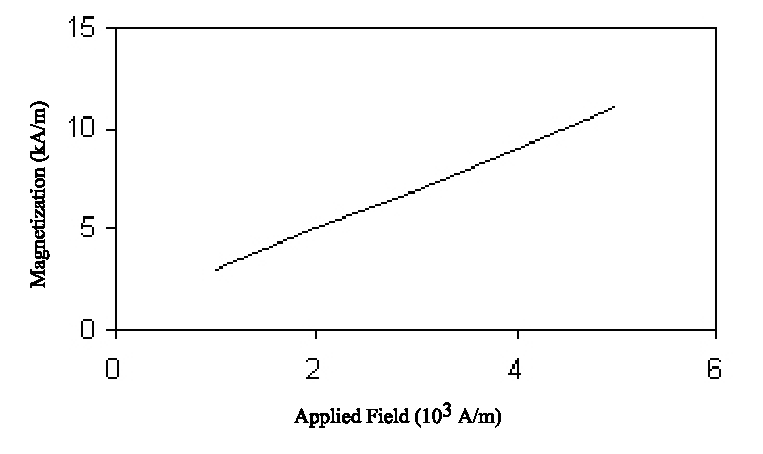
\includegraphics[width=3.2in]{imagen}
\caption{
Magnetization as a function of applied field. Note how the caption is centered in the column.
}
\label{fig_sim}
\end{figure}
\end{center}

\subsection{References}
Number citations consecutively in square brackets [1]. Punctuation
follows the bracket [2]. Refer simply to the reference number, as
in [3]. Use "Ref. [3]" or "Reference [3]" at the beginning of a
sentence: "Reference [3] was the first..."\\
\indent
Number footnotes
separately in superscripts. Place the actual footnote at the
bottom of the column in which it was cited. Do not put footnotes
in the reference list. Use letters for table footnotes (see Table
I). \textit{IEEE Transactions} no longer use a journal prefix before the
volume number. For example, use "\textit{IEEE Trans. Magn.}, vol. 25," not
"vol. MAG-25."\\
\indent
Give all authors' names; use "et al." if there are
six authors or more [4]. Papers that have not been published, even
if they have been submitted for publication, should be cited as
"unpublished" [4]. Papers that have been accepted for publication
should be cited as "in press" [5]. In a paper title, capitalize
the first word and all other words except for conjunctions,
prepositions less than seven letters, and prepositional phrases.\\
\indent
For papers published in translated journals, first give the
English citation, then the original foreign-language one [6].
\subsection{Abbreviations and Acronyms}
Define abbreviations and acronyms the first time they are used in
the text, even if they have been defined in the abstract.
Abbreviations such as IEEE, SI, MKS, CGS, ac, dc, and rms do not
have to be defined. Do not use abbreviations in the title unless
they are unavoidable.
\subsection{Equations}
Number equations consecutively with equation numbers in
parentheses flush with the right margin, as in (1). To make your
equations more compact, you may use the solidus (/) and the exp
function, etc. Italicize Roman symbols for quantities and
variables, but not Greek symbols. Use an en dash (-) rather than a
hyphen for a minus sign. Use parentheses to avoid ambiguities in
denominators. Punctuate equations with commas or periods when they
are part of a sentence, as in
\begin{equation}
\frac{e^{ix}}{2} = \frac{\cos{x}+i\sin{x}}{2}\Rightarrow \exp(ix)/2=(\cos{x}+i\sin{x})/2.
\label{ecuacion}
\end{equation}
Symbols in your equation should be defined before the equation
appears or immediately following. Cite equations using "(1)," not
Eq. (1)" or "equation (1)," except at the beginning of a sentence:
"Equation (1) is..."
\subsection{Other Recommendations}
The Roman numerals used to number the section headings are
optional. Do not number \textsc{Acknowledgment} and \textsc{References} and begin
Subheadings with letters. Use two spaces after periods (full
stops). Hyphenate complex modifiers: "zero-field-cooled
magnetization." Avoid dangling participles, such as, "Using (1),
the potential was calculated." Write instead, "The potential was
calculated using (1)," or "Using (1), we calculated the
potential."\\
Use a zero before decimal points:  "0.25," not ".25."
Use "cm$^{3}$," not "cc." Do not mix complete spellings and
abbreviations of units: "Wb/m$^{2}$" or "webers per square meter," not
"webers/m$^{2}$." Spell units when they appear in text: "�a few
henries," not "...a few H." If your native language is not English,
try to get a native English-speaking colleague to proofread your
paper. Do not add page numbers.

\section{Units}
Use either SI (MKS) or CGS as primary units. (SI units are
encouraged.) English units may be used as secondary units (in
parentheses). An exception would be the use of English units as
identifiers in trade, such as "3.5-inch disk drive."\\
\indent
Avoid combining SI and CGS units, such as current in amperes and
magnetic field in oersteds. This often leads to confusion because
equations do not balance dimensionally. If you must use mixed
units, clearly state the units for each quantity that you use in
an equation.

\section{Some Common Mistakes}
The word "data" is plural, not singular. In American English,
periods and commas are within quotation marks, like "this period."
A parenthetical statement at the end of a sentence is punctuated
outside of the closing parenthesis (like this). (A parenthetical
sentence is punctuated within the parentheses.) A graph within a
graph is an "inset," not an "insert." The word alternatively is
preferred to the word "alternately" (unless you mean something
that alternates). Do not use the word "essentially" to mean
"approximately" or "effectively." Be aware of the different
meanings of the homophones "affect" and "effect," "complement" and
"compliment," "discreet" and "discrete," "principal" and
"principle." Do not confuse "imply" and "infer." The prefix "non"
is not a word; it should be joined to the word it modifies,
usually without a hyphen. There is no period after the "et" in the
Latin abbreviation "et al." The abbreviation "i.e." means "that
is," and the abbreviation "e.g." means "for example."  An
excellent style manual for science writers is [7].

%\section{Conclusion}
% conference papers do not normally have an appendix

% use section* for acknowledgment
\section*{Acknowledgment}
% optional entry into table of contents (if used)
%\addcontentsline{toc}{section}{Acknowledgment}
The preferred spelling of the word "acknowledgment" in America is
without an "e" after the "g." Try to avoid the stilted expression,
"One of us (R. B. G.) thanks..." Instead, try "R.B.G. thanks..." Put
sponsor acknowledgments in the unnumbered footnote on the first
page.

% trigger a \newpage just before the given reference
% number - used to balance the columns on the last page
% adjust value as needed - may need to be readjusted if
% the document is modified later
%\IEEEtriggeratref{8}
% The "triggered" command can be changed if desired:
%\IEEEtriggercmd{\enlargethispage{-5in}}

% references section
\begin{thebibliography}{1}
%\bibitem{Bib:King}
%M. King, B. Zhu, and S. Tang, "Optimal path planning," Mobile Robots, vol. 8, no. 2, pp. 520-531, March 2001.
%\bibitem{Bib:Simpson}
%H. Simpson, Dumb Robots, 3rd ed., Springfield: UOS Press, 2004, pp.6-9.
\bibitem{Bib:King}
M. King and B. Zhu, "Gaming strategies," in Path Planning to the West, vol. II, S. Tang and M. King, Eds. Xian: Jiaoda Press, 1998, pp. 158-176.
\bibitem{Bib:Simpson}
B. Simpson, et al, "Title of paper goes here if known," unpublished.
\bibitem{Bib:Lu}
J.-G. Lu, "Title of paper with only the first word capitalized," J. Name Stand. Abbrev., in press.
\bibitem{Bib:Yorozu}
Y. Yorozu, M. Hirano, K. Oka, and Y. Tagawa, "Electron spectroscopy studies on magneto-optical media and plastic substrate interface," IEEE Translated J. Magn. Japan, vol. 2, pp. 740-741, August 1987 [Digest 9th Annual Conf. Magnetics Japan, p. 301, 1982].
\bibitem{Bib:Young}
M. Young, The Technical Writer's Handbook, Mill Valley, CA: University Science, 1989.
\end{thebibliography}

\end{document}
